\section{The Base}
\label{sec:base}

The program's aim is to find a discrete base from which space, time's arrow, relativity, spin, light, the quantum,
gravity and selves each come out, or to show the base is wrong \cite{pollard2026discrete, cluesurf2026repo}. It
draws on Margenstern's cellular automata in hyperbolic spaces \cite{margenstern2007vol1}. Every claim below is one
experiment in the suite, cited by its code (\code{E-SPN-0143} and so on), each with gates fixed before its run and
a computed control. A result is graded by depth: L1 is algebra, L2 a model run on the mesh, L3 the rule itself.

\subsection{Terms}

\begin{itemize}
\item \textbf{Tone.} One trit, $+1$, $0$ or $-1$. The whole state is tones. Three is the smallest alphabet with an
empty value and a sign flip, which is charge conjugation (\code{E-FND-0038}).
\item \textbf{Vibe.} A slot holding $+1$ (a \emph{love}) or $-1$ (a \emph{fear}). A slot holding 0 is calm. Charge
is love minus fear, content is love plus fear.
\item \textbf{Dock.} One site: 24 slots, one per root of $D_4$, the 24 vertices of a 24-cell. Opposite slots pair
into 12 \emph{lines}, and the lines fall into three \emph{frames} of four orthogonal lines. $D_4$ is the one 4d
root system with triality, and its 24 directions carry the spinor double cover, so a $2\pi$ turn gives $-1$
(\code{E-SPN-0042}).
\item \textbf{Mesh.} The space of docks. In the model it is $\{3,4,3,4\}$, whose vertex figure is the flat cubic
honeycomb $\{4,3,4\}$. It unfolds from one 24-cell in shells of 1, 24, 456, 8,376 and 153,192 docks, a ratio
settling at 18.278 (\code{E-GMT-0027}). Experiments run on a flat periodic $D_4$ box of side 8, 16 or 24, a
disclosed stand-in with the same 24 directions per dock.
\item \textbf{Beat.} One tick. Every dock applies the rule at once, so a run is reproducible bit for bit.
\item \textbf{Take.} Each beat a slot takes its neighbor's value along its root, the \emph{stream}. Nothing moves: a
value is read and written, never carried, so the stream is a permutation and runs backward exactly.
\item \textbf{Husk.} The three-dimensional surface where physics is read, the depth-even half of the box, exactly
closed (\code{E-FRC-0168}). In the honeycomb it is the flat horosphere at a cusp, and a spectral dimension near 3 is
read there (\code{E-GMT-0025}).
\item \textbf{Bulk, depth.} The 4d mesh behind the husk. A husk column is the stack of bulk docks behind one husk
dock, and its size $D$ is its depth. Every husk field is a column sum of bulk trits (\code{E-FRC-0207}).
\item \textbf{Role, link.} Each vibe carries a point on a 3 by 3 grid, a qutrit. A link between two docks holds one
of the 648 elements of the qutrit Clifford group $\Sigma(648)$ (\code{E-QTM-0117}). A link stores no matter: it is
the relation between the vibes on it.
\item \textbf{Store.} A dock line's held love and fear pair, made from an empty line and released back to it. This
is how the vacuum makes and unmakes pairs with its charge fixed at 0.
\item \textbf{Amplitude.} The state is a finite sum of configurations, each weighted by an exact number in
$\mathbb{Z}[\omega][1/2]$, $\omega = e^{2\pi i/3}$. Every three in the model lives in this ring, and nothing is
rounded.
\item \textbf{Path.} One measurement record of the quantum rule: at every split one branch, chosen by a deterministic
key. Fields are read as averages over paths.
\end{itemize}

\begin{figure}[ht]
\centering
\includegraphics[width=0.5\textwidth]{vibe-mesh-73}
\caption{The $\{7,3\}$ tessellation of the hyperbolic plane on the Poincar\'e disk, a two-dimensional stand-in for the
four-dimensional $\{3,4,3,4\}$, which cannot be pictured. Room opens faster than in flat space, which is what lets a
region's boundary act as a screen. The three colors mark the three values of a tone.}
\label{fig:mesh-73}
\end{figure}

\begin{figure}[ht]
\centering
\includegraphics[width=\textwidth]{vibe-mesh-534}
\caption{Inside the $\{5,3,4\}$ honeycomb of dodecahedra, the closest cousin that can be rendered in three
dimensions. It is a control, not the subject: its twelve directions carry no spinor, where the 24 directions of the
committed $\{3,4,3,4\}$ do.}
\label{fig:mesh-534}
\end{figure}

\subsection{The engine and the screen}

The claim has the shape of a video game. A small fixed engine updates a large state tick by tick, and what anyone
sees is a lossy projection of that state. Players learn a game's physics from the screen without reading its code,
and physics is that study of the screen. The program is a guess at the engine, one exact rule with no dice, tested by
running it and checking that it draws the screen we measure. The engine is the rule, which runs on every dock. The
bulk is part of the state, and the screen is the coarse-grained husk (Figure~\ref{fig:projection}). A coarse picture
is not a false one. The picture stops at the hardware: the mesh runs on nothing, and nobody plays.

\begin{figure}[ht]
\centering
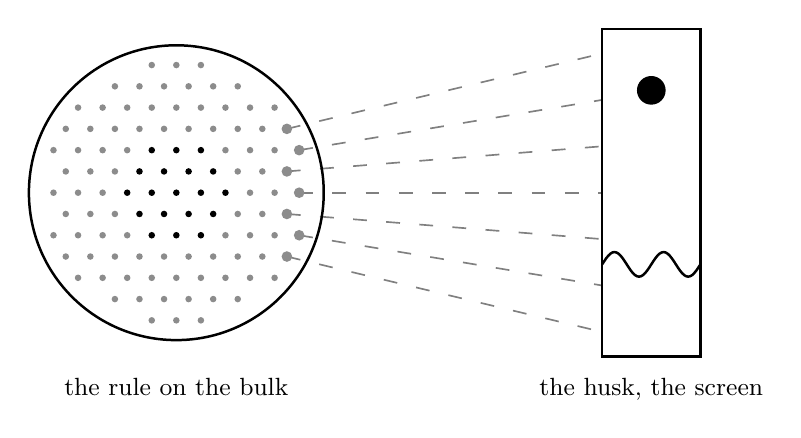
\begin{tikzpicture}[x=0.026cm,y=0.026cm]
\draw[line width=0.6pt, dash pattern=on 5 off 7, gray] (182.00,141.18) -- (336.00,178.00);
\draw[line width=0.6pt, dash pattern=on 5 off 7, gray] (188.00,130.78) -- (336.00,155.33);
\draw[line width=0.6pt, dash pattern=on 5 off 7, gray] (182.00,120.39) -- (336.00,132.67);
\draw[line width=0.6pt, dash pattern=on 5 off 7, gray] (188.00,110.00) -- (336.00,110.00);
\draw[line width=0.6pt, dash pattern=on 5 off 7, gray] (182.00,99.61) -- (336.00,87.33);
\draw[line width=0.6pt, dash pattern=on 5 off 7, gray] (188.00,89.22) -- (336.00,64.67);
\draw[line width=0.6pt, dash pattern=on 5 off 7, gray] (182.00,78.82) -- (336.00,42.00);
\draw[line width=0.9pt] (128.00,110.00) circle (72);
\fill[black!45] (116.00,172.35) circle (1.6);
\fill[black!45] (128.00,172.35) circle (1.6);
\fill[black!45] (140.00,172.35) circle (1.6);
\fill[black!45] (98.00,161.96) circle (1.6);
\fill[black!45] (110.00,161.96) circle (1.6);
\fill[black!45] (122.00,161.96) circle (1.6);
\fill[black!45] (134.00,161.96) circle (1.6);
\fill[black!45] (146.00,161.96) circle (1.6);
\fill[black!45] (158.00,161.96) circle (1.6);
\fill[black!45] (80.00,151.57) circle (1.6);
\fill[black!45] (92.00,151.57) circle (1.6);
\fill[black!45] (104.00,151.57) circle (1.6);
\fill[black!45] (116.00,151.57) circle (1.6);
\fill[black!45] (128.00,151.57) circle (1.6);
\fill[black!45] (140.00,151.57) circle (1.6);
\fill[black!45] (152.00,151.57) circle (1.6);
\fill[black!45] (164.00,151.57) circle (1.6);
\fill[black!45] (176.00,151.57) circle (1.6);
\fill[black!45] (74.00,141.18) circle (1.6);
\fill[black!45] (86.00,141.18) circle (1.6);
\fill[black!45] (98.00,141.18) circle (1.6);
\fill[black!45] (110.00,141.18) circle (1.6);
\fill[black!45] (122.00,141.18) circle (1.6);
\fill[black!45] (134.00,141.18) circle (1.6);
\fill[black!45] (146.00,141.18) circle (1.6);
\fill[black!45] (158.00,141.18) circle (1.6);
\fill[black!45] (170.00,141.18) circle (1.6);
\fill[black!45] (182.00,141.18) circle (2.6);
\fill[black!45] (68.00,130.78) circle (1.6);
\fill[black!45] (80.00,130.78) circle (1.6);
\fill[black!45] (92.00,130.78) circle (1.6);
\fill[black!45] (104.00,130.78) circle (1.6);
\fill[black] (116.00,130.78) circle (1.6);
\fill[black] (128.00,130.78) circle (1.6);
\fill[black] (140.00,130.78) circle (1.6);
\fill[black!45] (152.00,130.78) circle (1.6);
\fill[black!45] (164.00,130.78) circle (1.6);
\fill[black!45] (176.00,130.78) circle (1.6);
\fill[black!45] (188.00,130.78) circle (2.6);
\fill[black!45] (74.00,120.39) circle (1.6);
\fill[black!45] (86.00,120.39) circle (1.6);
\fill[black!45] (98.00,120.39) circle (1.6);
\fill[black] (110.00,120.39) circle (1.6);
\fill[black] (122.00,120.39) circle (1.6);
\fill[black] (134.00,120.39) circle (1.6);
\fill[black] (146.00,120.39) circle (1.6);
\fill[black!45] (158.00,120.39) circle (1.6);
\fill[black!45] (170.00,120.39) circle (1.6);
\fill[black!45] (182.00,120.39) circle (2.6);
\fill[black!45] (68.00,110.00) circle (1.6);
\fill[black!45] (80.00,110.00) circle (1.6);
\fill[black!45] (92.00,110.00) circle (1.6);
\fill[black] (104.00,110.00) circle (1.6);
\fill[black] (116.00,110.00) circle (1.6);
\fill[black] (128.00,110.00) circle (1.6);
\fill[black] (140.00,110.00) circle (1.6);
\fill[black] (152.00,110.00) circle (1.6);
\fill[black!45] (164.00,110.00) circle (1.6);
\fill[black!45] (176.00,110.00) circle (1.6);
\fill[black!45] (188.00,110.00) circle (2.6);
\fill[black!45] (74.00,99.61) circle (1.6);
\fill[black!45] (86.00,99.61) circle (1.6);
\fill[black!45] (98.00,99.61) circle (1.6);
\fill[black] (110.00,99.61) circle (1.6);
\fill[black] (122.00,99.61) circle (1.6);
\fill[black] (134.00,99.61) circle (1.6);
\fill[black] (146.00,99.61) circle (1.6);
\fill[black!45] (158.00,99.61) circle (1.6);
\fill[black!45] (170.00,99.61) circle (1.6);
\fill[black!45] (182.00,99.61) circle (2.6);
\fill[black!45] (68.00,89.22) circle (1.6);
\fill[black!45] (80.00,89.22) circle (1.6);
\fill[black!45] (92.00,89.22) circle (1.6);
\fill[black!45] (104.00,89.22) circle (1.6);
\fill[black] (116.00,89.22) circle (1.6);
\fill[black] (128.00,89.22) circle (1.6);
\fill[black] (140.00,89.22) circle (1.6);
\fill[black!45] (152.00,89.22) circle (1.6);
\fill[black!45] (164.00,89.22) circle (1.6);
\fill[black!45] (176.00,89.22) circle (1.6);
\fill[black!45] (188.00,89.22) circle (2.6);
\fill[black!45] (74.00,78.82) circle (1.6);
\fill[black!45] (86.00,78.82) circle (1.6);
\fill[black!45] (98.00,78.82) circle (1.6);
\fill[black!45] (110.00,78.82) circle (1.6);
\fill[black!45] (122.00,78.82) circle (1.6);
\fill[black!45] (134.00,78.82) circle (1.6);
\fill[black!45] (146.00,78.82) circle (1.6);
\fill[black!45] (158.00,78.82) circle (1.6);
\fill[black!45] (170.00,78.82) circle (1.6);
\fill[black!45] (182.00,78.82) circle (2.6);
\fill[black!45] (80.00,68.43) circle (1.6);
\fill[black!45] (92.00,68.43) circle (1.6);
\fill[black!45] (104.00,68.43) circle (1.6);
\fill[black!45] (116.00,68.43) circle (1.6);
\fill[black!45] (128.00,68.43) circle (1.6);
\fill[black!45] (140.00,68.43) circle (1.6);
\fill[black!45] (152.00,68.43) circle (1.6);
\fill[black!45] (164.00,68.43) circle (1.6);
\fill[black!45] (176.00,68.43) circle (1.6);
\fill[black!45] (98.00,58.04) circle (1.6);
\fill[black!45] (110.00,58.04) circle (1.6);
\fill[black!45] (122.00,58.04) circle (1.6);
\fill[black!45] (134.00,58.04) circle (1.6);
\fill[black!45] (146.00,58.04) circle (1.6);
\fill[black!45] (158.00,58.04) circle (1.6);
\fill[black!45] (116.00,47.65) circle (1.6);
\fill[black!45] (128.00,47.65) circle (1.6);
\fill[black!45] (140.00,47.65) circle (1.6);
\draw[line width=0.9pt] (336.00,30.00) rectangle (384.00,190.00);
\fill (360.00,160.00) circle (7);
\draw[line width=0.9pt] (336.00,75.00) -- (337.00,76.55) -- (338.00,78.00) -- (339.00,79.24) -- (340.00,80.20) -- (341.00,80.80) -- (342.00,81.00) -- (343.00,80.80) -- (344.00,80.20) -- (345.00,79.24) -- (346.00,78.00) -- (347.00,76.55) -- (348.00,75.00) -- (349.00,73.45) -- (350.00,72.00) -- (351.00,70.76) -- (352.00,69.80) -- (353.00,69.20) -- (354.00,69.00) -- (355.00,69.20) -- (356.00,69.80) -- (357.00,70.76) -- (358.00,72.00) -- (359.00,73.45) -- (360.00,75.00) -- (361.00,76.55) -- (362.00,78.00) -- (363.00,79.24) -- (364.00,80.20) -- (365.00,80.80) -- (366.00,81.00) -- (367.00,80.80) -- (368.00,80.20) -- (369.00,79.24) -- (370.00,78.00) -- (371.00,76.55) -- (372.00,75.00) -- (373.00,73.45) -- (374.00,72.00) -- (375.00,70.76) -- (376.00,69.80) -- (377.00,69.20) -- (378.00,69.00) -- (379.00,69.20) -- (380.00,69.80) -- (381.00,70.76) -- (382.00,72.00) -- (383.00,73.45) -- (384.00,75.00);
\node[below] at (128.00,24.00) {\small the rule on the bulk};
\node[below] at (360.00,24.00) {\small the husk, the screen};
\end{tikzpicture}

\caption{The engine and the screen. The rule runs on every dock of the bulk, drawn as a ball, and its activity
reaches the husk along rays. On the husk, the screen, it shows as what physics measures: a particle and a wave. On
the site the docks switch only on a beat while the projection flows. This is a still.}
\label{fig:projection}
\end{figure}

\subsection{Grading}

The working ledger lists 191 facts the model must produce, from the Born rule to the specious present, each graded
under one set of rules: read on the husk, the rule integer and reversible, a stand-in labeled and never graded as a
derivation, a numerical match counted only through a pre-registered null (\code{E-MTH-0010}), and the verdict judged
over 17 link starts (\code{E-MTH-0028}). Today 36 are held, 52 partial, 45 stand-in, 26 open and 32 not started. No
random number enters any run: starts, controls and nulls use Weyl sequences or enumeration.
